% !TEX program = xelatex
% 光遗传学与视觉功能恢复 · 四材料（选择题增强版，13 问 / 32 分）
% 编译：xelatex -interaction=nonstopmode -halt-on-error 本文件（跑两遍）
\documentclass[UTF8,a4paper,11pt]{ctexart}

\usepackage{geometry}
\geometry{left=1.9cm,right=1.9cm,top=2.3cm,bottom=2.3cm}
\usepackage{graphicx}
\usepackage{amsmath,amssymb}
\usepackage{booktabs}
\usepackage{longtable}
\usepackage{array}
\usepackage{enumitem}
\usepackage{xcolor}
\usepackage{caption}
\usepackage{float}
\usepackage{titlesec}
\usepackage{fancyhdr}
\usepackage{tcolorbox}
\tcbuselibrary{skins,breakable}
\usepackage[hidelinks]{hyperref}

\graphicspath{{../命题图/}{../../Resources/Downloads/原图-光遗传学视觉恢复/}}

\definecolor{deepblue}{HTML}{1F4E79}
\definecolor{deepred}{HTML}{C00000}
\definecolor{deepgreen}{HTML}{2E7D32}

\captionsetup{font=small,labelfont=bf,skip=4pt}
\titleformat{\section}{\Large\bfseries\color{deepblue}}{\thesection}{0.6em}{}
\titleformat{\subsection}{\normalsize\bfseries\color{deepblue}}{\thesubsection}{0.6em}{}
\pagestyle{fancy}
\fancyhf{}
\fancyhead[L]{\small 光遗传学与视觉功能恢复 · 四材料十三问（32 分）}
\fancyhead[R]{\small\thepage}

\newcommand{\pt}[1]{\textbf{（#1分）}}
\newcommand{\lv}[1]{{\small\color{deepgreen}［#1］}}
\newcommand{\key}[1]{\textbf{\color{deepred}#1}}
\newcommand{\tian}[1]{\underline{\hspace{#1}}}
\newcommand{\choice}[1]{\par\smallskip\noindent #1\par}

% 材料区块：位于材料开头；设问区块：紧跟对应材料
\newtcolorbox{matbox}[1]{colback=blue!4,colframe=deepblue,boxrule=0.9pt,
  arc=2pt,left=6pt,right=6pt,top=5pt,bottom=5pt,
  title={\bfseries #1},fonttitle=\normalsize\color{white},
  coltitle=white,colbacktitle=deepblue,breakable}
\newtcolorbox{qbox}{colback=deepgreen!5,colframe=deepgreen,boxrule=0.7pt,
  arc=2pt,left=6pt,right=6pt,top=4pt,bottom=4pt,breakable,
  before skip=6pt,after skip=6pt}

\title{\bfseries 光遗传学与视网膜退化性疾病的视觉功能恢复\\[5pt]
\large 四材料综合题 · 选择题增强版（13 问 / 32 分）}
\author{}\date{2026-10-06}

\begin{document}
\maketitle
\thispagestyle{fancy}

\begin{center}
\fbox{\parbox{0.95\textwidth}{\small
\textbf{阅读提示}：科研事实取自 Pan et al. 2014、Lu et al. 2016、Lu et al. 2018 三篇开放获取论文。
专业名词均在材料或表注中给出\textbf{做题所需的解释}，不需事先记忆；标"\key{命题简化}"的数据，数值为命题需要而设定，\emph{趋势}依原论文改写。
\textbf{题型}：单选 2、多选 4、编号选填 1、编号排序 1，\textbf{客观题 8 问共 15 分}；简答与分析 5 问共 17 分。
}}
\end{center}

\section*{命题说明}
\addcontentsline{toc}{section}{命题说明}

\begin{table}[H]
\centering\small
\begin{tabular}{@{}llcccc@{}}
\toprule
\textbf{题号} & \textbf{题型} & \textbf{考查落点} & \textbf{难度} & \textbf{分值} & \textbf{材料} \\
\midrule
Q1 & 单选 & 视网膜细胞分工与损伤部位 & 基础 & 2 & 一 \\
Q2 & 多选 & RP 与光遗传学治疗的性质辨析 & 基础 & 2 & 一 \\
Q3 & 简答 & 信号通路中断的后果 & 基础 & 3 & 一 \\
Q4 & 编号排序 & 据表比较被弱光激活的能力 & 基础 & 2 & 二 \\
Q5 & 多选 & 被弱光激活的能力与恢复时间的关系 & 中等 & 2 & 二 \\
Q6 & 简答 & 多指标权衡（优势与局限） & 拔高 & 3 & 二 \\
Q7 & 编号选填+简答 & 据表选择方案并说明理由 & 中等 & 3 & 三 \\
Q8 & 多选 & 载体与调控元件的功能 & 中等 & 2 & 三 \\
Q9 & 简答 & 表达量 ≠ 功能（层次差异） & 拔高 & 3 & 三 \\
Q10 & 单选 & 据表判断视觉功能恢复最好者 & 中等 & 2 & 四 \\
Q11 & 多选 & 对照与评价指标 & 拔高 & 2 & 四 \\
Q12 & 简答 & 实验变量分析＋对照的作用 & 中等 & 3 & 四 \\
Q13 & 简答·开放 & 综合方案与依据 & 拔高 & 3 & 综合 \\
\midrule
\multicolumn{4}{r}{\textbf{合计}} & \textbf{32} & \\
\bottomrule
\end{tabular}
\end{table}

\noindent\textbf{难度分层}：基础 9 分；中等 11 分；拔高 12 分。\textbf{主要区分点}：Q6（多指标权衡）、Q9（表达量≠功能）、Q13（综合评价）。

\section{材料一\quad 视觉损伤与治疗思路}
\addcontentsline{toc}{section}{材料一：视觉损伤与治疗思路}

\begin{matbox}{材料一\quad 视觉损伤与治疗思路}
视网膜像一台"光信号转换器"：其中的\textbf{感光细胞}（视杆细胞与视锥细胞）感受光并把光信号转变为电信号；信号随后经\textbf{双极细胞}传到\textbf{神经节细胞}，后者的轴突汇聚成视神经，把信号送往大脑皮层视觉中枢，最终形成视觉（图1）。

视网膜色素变性（RP）是一类由基因突变引起的遗传性眼病。患者的\textbf{感光细胞逐渐死亡}，而内层的双极细胞与神经节细胞大多仍然存活。由于信号在视网膜的"第一站"就无法形成，患者即使眼球结构和视神经通路完好，视觉功能仍会逐渐下降。

研究者尝试用\textbf{光遗传学}方法恢复视觉：把一种来自单细胞藻类的\textbf{光敏蛋白基因（ChR2 基因）}导入残存的视网膜细胞。ChR2 蛋白能在细胞膜上形成\textbf{受光控制的离子通道}——受到蓝光照射时通道开放，离子流动，细胞的膜电位随之改变，从而产生电信号。
\end{matbox}

\begin{figure}[H]
\centering
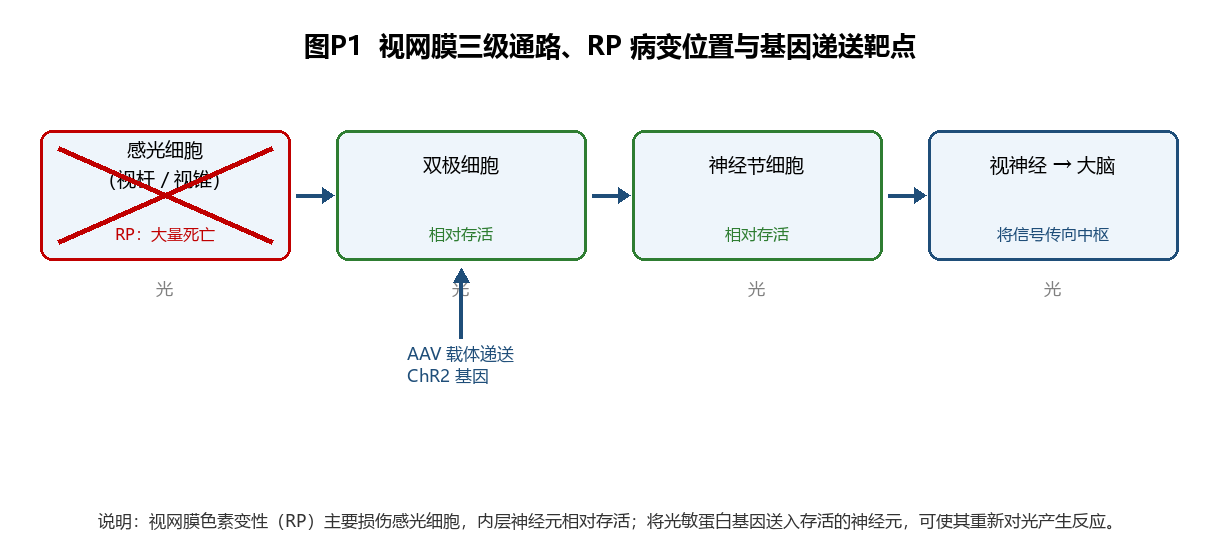
\includegraphics[width=0.6\textwidth]{P1_视网膜三级通路与病变.png}
\caption{图1\quad 视网膜三级细胞通路、RP 的主要受损环节与治疗靶点（简化示意图）}
\end{figure}

\begin{qbox}
\noindent\textbf{\color{deepgreen}第 1—4 问（据材料一作答）}
\begin{enumerate}[leftmargin=2.2em,itemsep=5pt]
\item \lv{单选} \pt{2} 结合图1 与材料，RP 患者视觉功能下降的直接原因是（\quad）\\
\choice{A. 视神经被切断，信号无法上传到大脑\\
B. 感光细胞死亡，光信号无法在视网膜内被转变为神经信号\\
C. 双极细胞与神经节细胞也大量死亡，视网膜无法传递信号\\
D. 大脑皮层的视觉中枢受损，无法形成视觉}

\item \lv{多选} \pt{2} 结合材料，关于 RP 与光遗传学治疗，下列说法合理的有（\quad）（错选得 0 分）\\
\choice{A. RP 患者感光细胞大量死亡，而双极细胞与神经节细胞大多存活\\
B. 把 ChR2 基因导入残存神经细胞后，这些细胞在蓝光照射下可产生电位变化\\
C. 光遗传学治疗从根本上修复了患者致病的基因，因此可治愈 RP\\
D. 治疗后视觉信号仍需经神经节细胞传至大脑皮层视觉中枢才能形成视觉}

\item \lv{基础} \pt{3} 根据材料与图1，分析感光细胞退化为什么会引起视觉功能下降。

\item \lv{中等} \pt{3} 研究者把 ChR2 基因导入残存的视网膜神经细胞后，这些细胞便能在蓝光照射下产生反应。请用"基因 → 蛋白质 → 细胞功能"的思路说明其原因。
\end{enumerate}
\end{qbox}

\section{材料二\quad ChR2 突变体}
\addcontentsline{toc}{section}{材料二：ChR2 突变体}

\begin{matbox}{材料二\quad ChR2 突变体}
天然 ChR2 需要较强的光才能被有效激活。研究者通过改变 ChR2 基因中特定位置的碱基序列，获得三种突变体，并比较了它们的性能（表1）。
\end{matbox}

\begin{table}[H]
\centering\small
\caption*{\textbf{表1}\quad ChR2 及其突变体的性能比较（\key{命题简化}数据）}
\begin{tabular}{@{}lccc@{}}
\toprule
\textbf{变体} & \textbf{引起光响应所需的最低光强} & \textbf{光照停止后恢复到静息所需时间} & \textbf{在快速闪烁光下的响应} \\
\midrule
wt-ChR2（未改造） & 12 & 短 & 好 \\
M1（ChR2-L132C） & 5 & 中 & 中 \\
M2（ChR2-L132C/T159C） & 2 & 长 & 差 \\
M3（ChR2-L132C/T159S） & 3 & 很长 & 很差 \\
\bottomrule
\end{tabular}

\smallskip
\parbox{0.94\textwidth}{\footnotesize 注："引起光响应所需的最低光强"数值越小，表示细胞在越弱的光下即可被激活；"恢复到静息所需时间"越长，表示细胞在光照停止后越难迅速恢复，对随时间快速变化的光信号跟随能力越弱。数据为命题简化，趋势依据 Pan et al., 2014 改写。}
\end{table}

\subsection*{问题}

\begin{qbox}
\noindent\textbf{\color{deepgreen}第 5—7 问（据材料二作答）}
\begin{enumerate}[leftmargin=2.2em,itemsep=5pt,start=5]
\item \lv{编号排序} \pt{2} 根据表1，把四种变体按\textbf{被弱光激活的能力由强到弱}排序（填变体名称）：\\
\tian{2.4cm} $>$ \tian{2.4cm} $>$ \tian{2.4cm} $>$ \tian{2.4cm}

\item \lv{多选} \pt{2} 据表1，下列说法正确的有（\quad）（错选得 0 分）\\
\choice{A. M2 引起光响应所需的光强最低，在弱光下最容易被激活\\
B. 被弱光激活的能力越强的变体，恢复到静息所需的时间越短\\
C. 在快速闪烁光下响应最好的变体是 wt-ChR2\\
D. 表1 显示，"被弱光激活的能力"与"恢复时间"总体相关，但并非严格对应}

\item \lv{拔高} \pt{3} 某突变体被弱光激活的能力明显提高，但光照停止后恢复到静息所需时间变长。请结合表1 分析它用于视觉恢复时的\textbf{优势}与\textbf{局限}，并说明"被弱光激活的能力最强"是否就等于"视觉恢复效果最好"。
\end{enumerate}
\end{qbox}

\section{材料三\quad AAV 递送与目标细胞表达}
\addcontentsline{toc}{section}{材料三：AAV 递送与目标细胞表达}

\begin{matbox}{材料三\quad AAV 递送与目标细胞表达}
把基因送入细胞需要"载体"。研究者使用\textbf{腺相关病毒（AAV）}作为载体：它能把携带的基因送入细胞，且本身引起的免疫反应较弱。但仅有载体还不够——基因在哪些细胞里表达、表达多少，与连接在它旁边的\textbf{调控元件}（启动子、增强子）有关：它们能影响目的基因在不同细胞中的表达水平。

研究者设计了三种构建方案（方法中只有调控元件不同），并检测了小鼠视网膜中的表达情况（表2）。图2 是把 ChR2 与红色荧光蛋白融合后，与能标记双极细胞的抗体共同染色的结果：若红色荧光（表示基因表达）与绿色荧光（表示双极细胞）大量重叠，说明目的基因主要表达在双极细胞中。
\end{matbox}

\begin{table}[H]
\centering\small
\caption*{\textbf{表2}\quad 三种构建方案的表达情况比较（\key{命题简化}数据）}
\begin{tabular}{@{}lccc@{}}
\toprule
\textbf{方案} & \textbf{ChR2 总表达量} & \textbf{双极细胞中表达比例} & \textbf{非目标细胞中表达情况} \\
\midrule
甲 & 高 & 低 & 明显 \\
乙 & 中 & 高 & 很少 \\
丙 & 低 & 很高 & 极少 \\
\bottomrule
\end{tabular}

\smallskip
\parbox{0.94\textwidth}{\footnotesize 注：三种方案的目的是相同的（让视网膜细胞获得光响应），区别只在调控元件。数据为命题简化，趋势依据 Lu et al., 2016 结果改写。}
\end{table}

\begin{figure}[H]
\centering
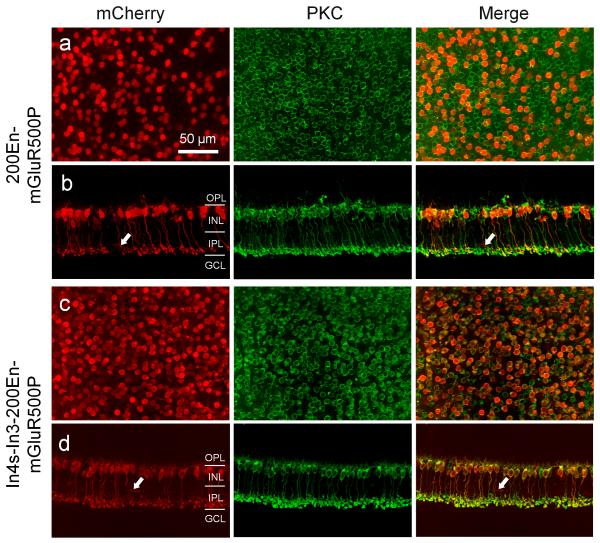
\includegraphics[width=0.52\textwidth]{Lu2016-Fig04.jpg}
\caption{图2\quad 论文原图（Lu et al., 2016）：目的基因表达产物（红）与双极细胞标记物（绿）的重叠情况}
\end{figure}

\subsection*{问题}

\begin{qbox}
\noindent\textbf{\color{deepgreen}第 8—10 问（据材料三作答）}
\begin{enumerate}[leftmargin=2.2em,itemsep=5pt,start=8]
\item \lv{编号选填+简答} \pt{3}
\begin{enumerate}[label=(\arabic*),leftmargin=1.4em,itemsep=2pt]
\item 若要使目的基因\textbf{主要在双极细胞中表达}，应选择表2 中的方案\tian{0.8cm}（填"甲""乙"或"丙"）（1 分）
\item 说明你的判断理由（2 分）。
\end{enumerate}

\item \lv{多选} \pt{2} 关于 AAV 载体与调控元件，下列说法正确的有（\quad）（错选得 0 分）\\
\choice{A. AAV 的作用是把目的基因送入细胞，属于基因工程中的载体\\
B. 调控元件能影响目的基因在哪些细胞中表达以及表达量的高低\\
C. 只要提高 ChR2 的总表达量，就一定能提高视觉恢复效果\\
D. 目的基因若在非目标细胞中大量表达，可能干扰视网膜原有的信号处理}

\item \lv{拔高} \pt{3} 表2 中甲方案的 ChR2 总表达量最高，但研究者并未选择它。请结合表1—表3，说明为什么"ChR2 表达量高"不能说明视觉恢复效果好。
\end{enumerate}
\end{qbox}

\section{材料四\quad 用 OMR 评价视觉功能是否恢复}
\addcontentsline{toc}{section}{材料四：用 OMR 评价视觉功能是否恢复}

\begin{matbox}{材料四\quad 用 OMR 评价视觉功能是否恢复}
细胞"对光有反应"不等于动物"看得见"。为评价视觉功能是否真正恢复，研究者使用\textbf{视动反应（OMR）}：把小鼠放在能显示移动条纹的装置中，若小鼠能看清条纹，其头部会随条纹运动方向转动；条纹越密集（\textbf{空间频率}越高），看清越困难，需要的光也越强。

研究者把三种 ChR2 变体分别导入三组同种失明小鼠，并设置一组\textbf{未经基因治疗}的小鼠作对照，测定了各组出现 OMR 所需的最低光强（表3）。
\end{matbox}

\begin{table}[H]
\centering\small
\caption*{\textbf{表3}\quad 各组小鼠出现 OMR 所需的最低光强（\key{命题简化}数据；"未出现"表示该条件下测不到 OMR）}
\begin{tabular}{@{}lccc@{}}
\toprule
\textbf{组别} & \textbf{条纹稀疏} & \textbf{条纹中等} & \textbf{条纹密集} \\
\midrule
未经基因治疗的对照组 & 未出现 & 未出现 & 未出现 \\
wt-ChR2 组 & 25 & 未出现 & 未出现 \\
M1 组 & 12 & 20 & 28 \\
M2 组 & 5 & 8 & 40 \\
M3 组 & 6 & 14 & 未出现 \\
\bottomrule
\end{tabular}
\end{table}

\subsection*{问题}

\begin{qbox}
\noindent\textbf{\color{deepgreen}第 11—12 问（据材料四作答）}
\begin{enumerate}[leftmargin=2.2em,itemsep=5pt,start=11]
\item \lv{单选} \pt{2} 在条纹稀疏与中等两种条件下，出现 OMR 所需最低光强最小（最容易被测到 OMR）的一组是（\quad）\\
\choice{A. wt-ChR2 组 \quad B. M1 组 \quad C. M2 组 \quad D. M3 组}

\item \lv{多选} \pt{2} 关于该实验，下列说法正确的有（\quad）（错选得 0 分）\\
\choice{A. 设置未经基因治疗的对照组，可用于排除其他因素引起 OMR 的可能\\
B. 各组小鼠的遗传背景、载体注射量与测定时间应保持一致\\
C. 视网膜中 ChR2 表达量越高，说明视觉恢复效果一定越好\\
D. OMR 是否出现属于行为学指标，比单纯检测蛋白表达更能反映视觉功能}

\item \lv{中等} \pt{3} 请回答下列两个问题：
\begin{enumerate}[label=(\arabic*),leftmargin=1.4em,itemsep=2pt]
\item \pt{2} 若研究目的是"比较两种 ChR2 突变体对视觉恢复的影响"，请写出该实验的\textbf{自变量}、\textbf{因变量}，以及至少两个需要控制相同的变量。
\item \pt{1} 为什么必须设置"未经基因治疗"的对照组？若该对照组也出现了 OMR，最可能说明什么？
\end{enumerate}
\end{enumerate}
\end{qbox}

\section{综合题}
\addcontentsline{toc}{section}{综合题}

\begin{qbox}
\noindent\textbf{\color{deepgreen}第 13 问（综合全部材料作答）}
\begin{enumerate}[leftmargin=2.2em,itemsep=5pt,start=13]
\item \lv{拔高·开放} \pt{3} 有一位患者以\textbf{夜间活动为主}，且需要\textbf{躲避快速移动的物体}。请综合表1—表3 的结果，从"\textbf{变体选择}、\textbf{靶细胞表达}、\textbf{功能评价}"中至少两个方面提出你的方案，并说明依据。
\end{enumerate}
\end{qbox}

\clearpage
\section*{参考答案与评分细则}
\addcontentsline{toc}{section}{参考答案与评分细则}

\begin{longtable}{@{}p{0.9cm}p{9.6cm}p{4.2cm}@{}}
\toprule
\textbf{题} & \textbf{参考答案} & \textbf{评分点} \\
\midrule
\endhead
Q1 & \textbf{B}。材料说明内层神经元大多存活，故 C 错；A、D 与"视神经通路与视觉中枢完好"不符。 & 选 B 得 2 分，其余 0 分。 \\
\addlinespace
Q2 & \textbf{ABD}。C 错：光遗传学并未修复致病基因，而是让残存细胞获得光响应能力，属于功能补偿，不是根治。 & 选 ABD 得 2 分；选 AB、AD、BD 得 1 分；含 C 得 0 分。 \\
\addlinespace
Q3 & 感光细胞是视网膜形成视觉信号的\textbf{第一站}，其功能是把光信号转变为电信号；感光细胞退化死亡后，光信号无法被转换，位于其下游的双极细胞、神经节细胞虽存活却\textbf{得不到输入}，视网膜无法向大脑输出信号，故视觉功能下降。 & 说出感光细胞的功能 1 分；指出信号在视网膜第一站中断 1 分；体现"下游细胞存活但无输入"1 分。仅答"细胞死了"不得分。 \\
\addlinespace
Q4 & M2 $>$ M3 $>$ M1 $>$ wt-ChR2（按所需最低光强由小到大，即由强到弱）。 & 顺序完全正确得 2 分；错误或漏项得 0 分。 \\
\addlinespace
Q5 & \textbf{ACD}。B 错：表1 显示被弱光激活能力越强的变体，恢复到静息所需时间越长，二者关系相反；D 对：二者总体相关但并非严格对应（M3 所需光强略高于 M2，恢复时间却更长）。 & 选 ACD 得 2 分；选 A、C、D、AC、AD、CD 得 1 分；含 B 得 0 分。 \\
\addlinespace
Q6 & \textbf{优势}：该突变体引起光响应所需的光强最低，即在很弱的光下即可被激活，适合弱光环境（夜间、室内）使用。\textbf{局限}：光照停止后恢复到静息所需时间最长，对随时间快速变化的光信号（快速闪烁、运动）跟随能力最差，动态视觉信息可能难以分辨。\textbf{结论}：被弱光激活的能力强只意味着"更容易被激活"，视觉恢复还要求能分辨随时间变化的信息，故"最强"不等于"最好"，需在多指标间权衡。 & 优势 1 分；局限 1 分；得出"需权衡、最强≠最好"1 分。只答"它更敏感"不得分。 \\
\addlinespace
Q7 & (1) \textbf{丙}。(2) 丙方案在目标细胞（双极细胞）中的表达比例最高、在非目标细胞中表达极少，说明目的基因被尽量限制在双极细胞中表达，\textbf{细胞特异性最好}；甲方案虽然总表达量最高，但在非目标细胞中表达明显，不能达到"主要在双极细胞中表达"的目的。 & (1) 填"丙"1 分。(2) "双极细胞中表达比例最高"1 分；"非目标细胞中表达极少（特异性好）"或"指出甲的高表达量不等于特异性"1 分。 \\
\addlinespace
Q8 & \textbf{ABD}。C 错：总表达量提高只说明产生了更多 ChR2 蛋白，若表达在非目标细胞中或蛋白功能（如恢复时间）不合适，视觉恢复效果未必更好。 & 选 ABD 得 2 分；选 AB、AD、BD 得 1 分；含 C 得 0 分。 \\
\addlinespace
Q9 & 不充分。①"ChR2 总表达量"只说明细胞内产生了多少 ChR2 蛋白，属于\textbf{蛋白质水平}的信息；② 甲方案虽总表达量最高，但在非目标细胞中表达明显（表2），这些细胞即使产生 ChR2 也未必形成有效视觉信号，还可能干扰视网膜原有的信号处理；③ 表1、表3 表明，即使表达了蛋白，若其\textbf{恢复时间过长}（如 M3），动物在行为上仍可能测不到 OMR。因此从蛋白质水平→细胞水平→行为（功能）水平存在层次差异，视觉恢复效果最终须由\textbf{行为学功能指标}评价。 & 指出表达量属蛋白质水平、为必要而非充分条件 1 分；结合表2 说明 1 分；结合表1／表3 或明确"须以行为学功能为最终标准"1 分。 \\
\addlinespace
Q10 & \textbf{C}（M2 组）。该组在条纹稀疏、中等条件下所需最低光强（5、8）均小于其他组。 & 选 C 得 2 分；其余 0 分。 \\
\addlinespace
Q11 & \textbf{ABD}。C 错：表3 显示各组都能表达 ChR2，但所需最低光强明显不同（M2 在密集条纹下反而不如 M1），说明表达量不能代表视觉功能恢复程度。 & 选 ABD 得 2 分；选 AB、AD、BD 得 1 分；含 C 得 0 分。 \\
\addlinespace
Q12 & (1) \textbf{自变量}：导入的 ChR2 变体种类（并设未经基因治疗的对照组）；\textbf{因变量}：是否出现 OMR、出现 OMR 所需的最低光强；\textbf{需控制相同的变量}（答两个）：小鼠的遗传背景与生理状态、注射的载体量与浓度、注射后至测定的时间、条纹移动速度与光刺激条件。(2) 对照用于排除"失明小鼠自身残留的光感受能力、注射操作或光刺激"等因素引起 OMR 的可能，说明观察到的 OMR 确实由导入的 ChR2 引起；若对照组也出现 OMR，则说明该反应不是（或不只是）由 ChR2 引起——可能小鼠并未真正失去光感受能力（模型不纯）或判定标准过宽，应先检验模型、重设判定标准后再作结论。 & (1) 自变量 1 分（须含对照）；因变量 0.5 分；控制变量两个 0.5 分。(2) 对照作用 0.5 分；指出"并非由 ChR2 引起／模型不纯"0.5 分。 \\
\addlinespace
Q13 & \textbf{（示例，答出"两个方面＋依据"即可）}\newline
\textbf{① 变体选择}：夜间活动需要弱光下即可被激活，表3 中 M2 在条纹稀疏、中等时所需光强最低（5、8）；但 M2 恢复到静息所需时间最长，在条纹密集（对应快速移动物体）时所需光强反而高于 M1（40 与 28），说明它分辨快速移动物体的能力较弱。因此若最看重夜间看清环境可选 M2，若最看重辨识快速移动物体可考虑 M1。\newline
\textbf{② 靶细胞表达}：选择表2 中丙（或乙）方案，使 ChR2 尽量只在双极细胞中表达，减少非目标细胞表达及其对原有信号的干扰。\newline
\textbf{③ 功能评价}：不能只用一种条件评价疗效，应同时测定条纹稀疏与密集条件下的 OMR，并增加如瞳孔对光收缩等其他指标。\newline
\textbf{结论}：视觉恢复需综合考虑被弱光激活的能力、恢复时间、靶细胞表达、非目标细胞表达以及行为水平的功能表现。 & 结合"夜间（弱光）"与"移动物体（快速变化）"两个需求并引用表3 数据 1 分；指出 M2 与 M1 的取舍关系 1 分；从至少两个方面提出方案且合理 0.5 分；得出"需综合多指标"的结论 0.5 分。 \\
\bottomrule
\end{longtable}

\section*{命题底线自检}
\addcontentsline{toc}{section}{命题底线自检}

\begin{longtable}{@{}p{0.6cm}p{6.0cm}p{8.2cm}@{}}
\toprule
\textbf{\#} & \textbf{底线要求} & \textbf{落实情况} \\
\midrule
\endhead
1 & 不要求学生背诵 ChR2、mGluR6、AAV 的专业定义 & 均以"材料给定的含义"出现；选择题只考其\emph{功能角色}，不考定义式记忆。 \\
\addlinespace
2 & 首次出现的专业事实必须给出必要解释 & 最低光强、恢复到静息所需时间、空间频率、OMR、调控元件、共同染色等均在材料或表注中解释。 \\
\addlinespace
3 & 不使用大学电生理学作为直接考点 & 未要求解释动作电位的离子机制；"恢复时间"只作表中信息用于比较。 \\
\addlinespace
4 & 不要求记忆实验编号、载体编号、品系名称 & 全文无载体编号、血清型与小鼠品系名称（变体以 M1—M3 代号出现，含义已在表1 注明）。 \\
\addlinespace
5 & 专业数据经过高中化处理 & 表1—表3 均为相对值并标注"命题简化"，趋势依原文改写。 \\
\addlinespace
6 & 高难度来自多证据整合 & Q6（表1 两列指标权衡）、Q9（表1＋表2＋表3 整合）、Q13（四段材料整合）难点均在证据整合与变量分析。 \\
\addlinespace
7 & 每个结论都有材料或高中知识支持 & 逐问核查：Q1—Q4（图1＋材料一）、Q5—Q7（表1）、Q8—Q10（表2＋图2）、Q11—Q13（表3）。 \\
\bottomrule
\end{longtable}

\section*{附录\quad 论文原图对照（课堂延伸用）}
\addcontentsline{toc}{section}{附录：论文原图对照}

\begin{figure}[H]
\centering
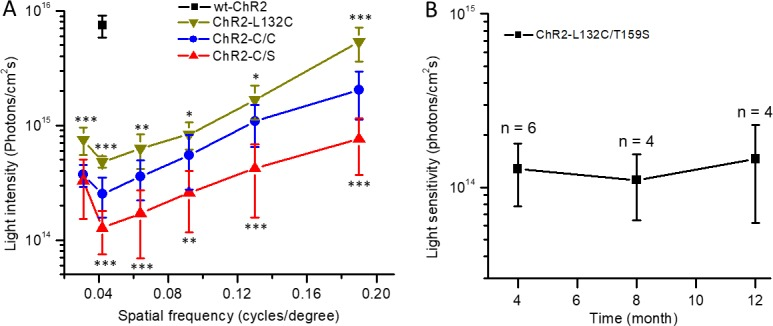
\includegraphics[width=0.68\textwidth]{Lu2018-Fig04.jpg}
\caption{图A\quad 论文原图（Lu et al., \textit{IOVS}, 2018, Fig.~4）：三种 ChR2 变体的 OMR 阈值光强—空间频率关系，与表3 的设计思路一致，供课堂延伸或按真实数据替换表3 时对照使用。}
\end{figure}

\noindent\small 全部 22 张论文原图与三篇文献存于 \texttt{00 - Personal/Resources/Downloads/}。

\end{document}
